{
\begin{frame}
    \begin{block}{}
        \begin{center}
            Prepare for launch!
        \end{center}
    \end{block}
\end{frame}
\usebackgroundtemplate{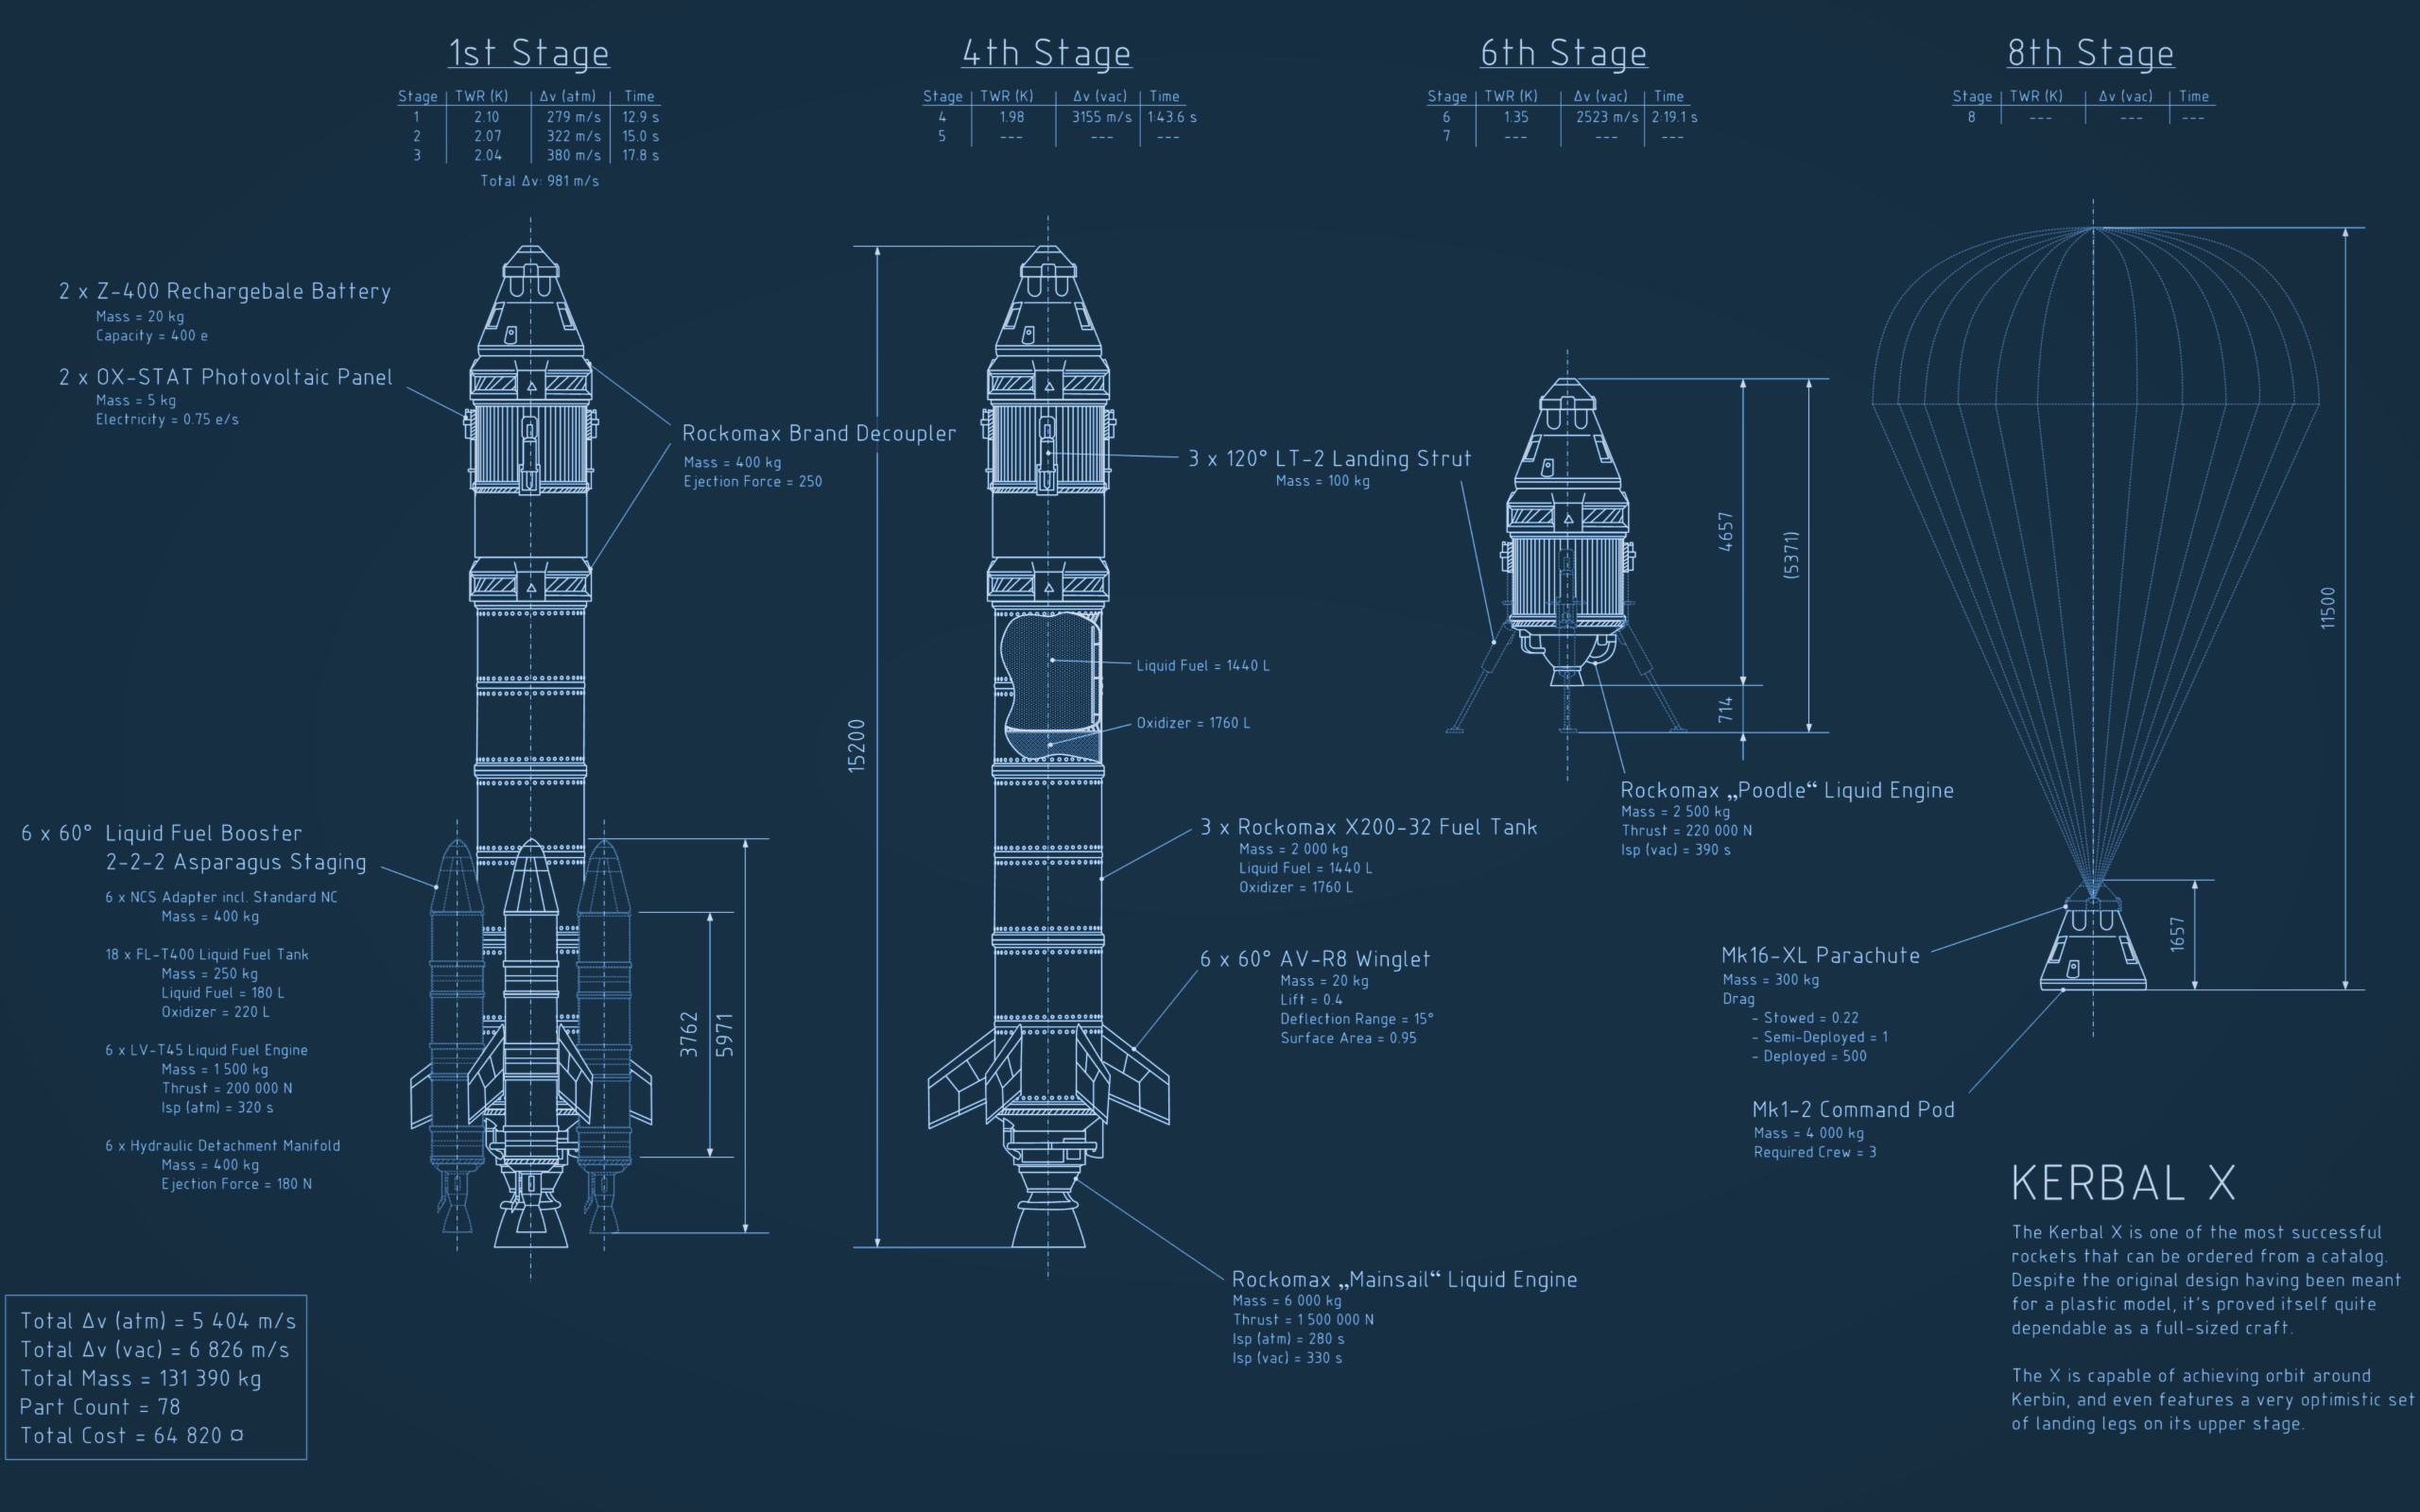
\includegraphics[height=\paperheight,keepaspectratio]{images/staging}}%
\begin{frame}
    \frametitle{Staging}
\end{frame}
\begin{frame}
    \frametitle{Staging}
    \begin{block}{How do we do it}
        \begin{itemize}
            \item Split the rocket in different parts (stages).
            \item Each stage carries its own fuel and engine, and can be separated from the rocket in sequence
            \item For instance: booster stage, transfer stage, landing stage, ...
        \end{itemize}
    \end{block}
\end{frame}
\begin{frame}
    \frametitle{Staging}
    \begin{block}{Why do we do it}
        \begin{itemize}
            \item Rocket efficiency is inversely proportional to its weight
            \item Delta-v goes up as total mass decreases, so we want to carry as little mass as posible
            \item Throw away excess weight of unused engines and empty fuel tanks
        \end{itemize}
    \end{block}
\end{frame}
}
\begin{frame}
    \frametitle{Staging}
    \begin{block}{}
        \begin{center}
            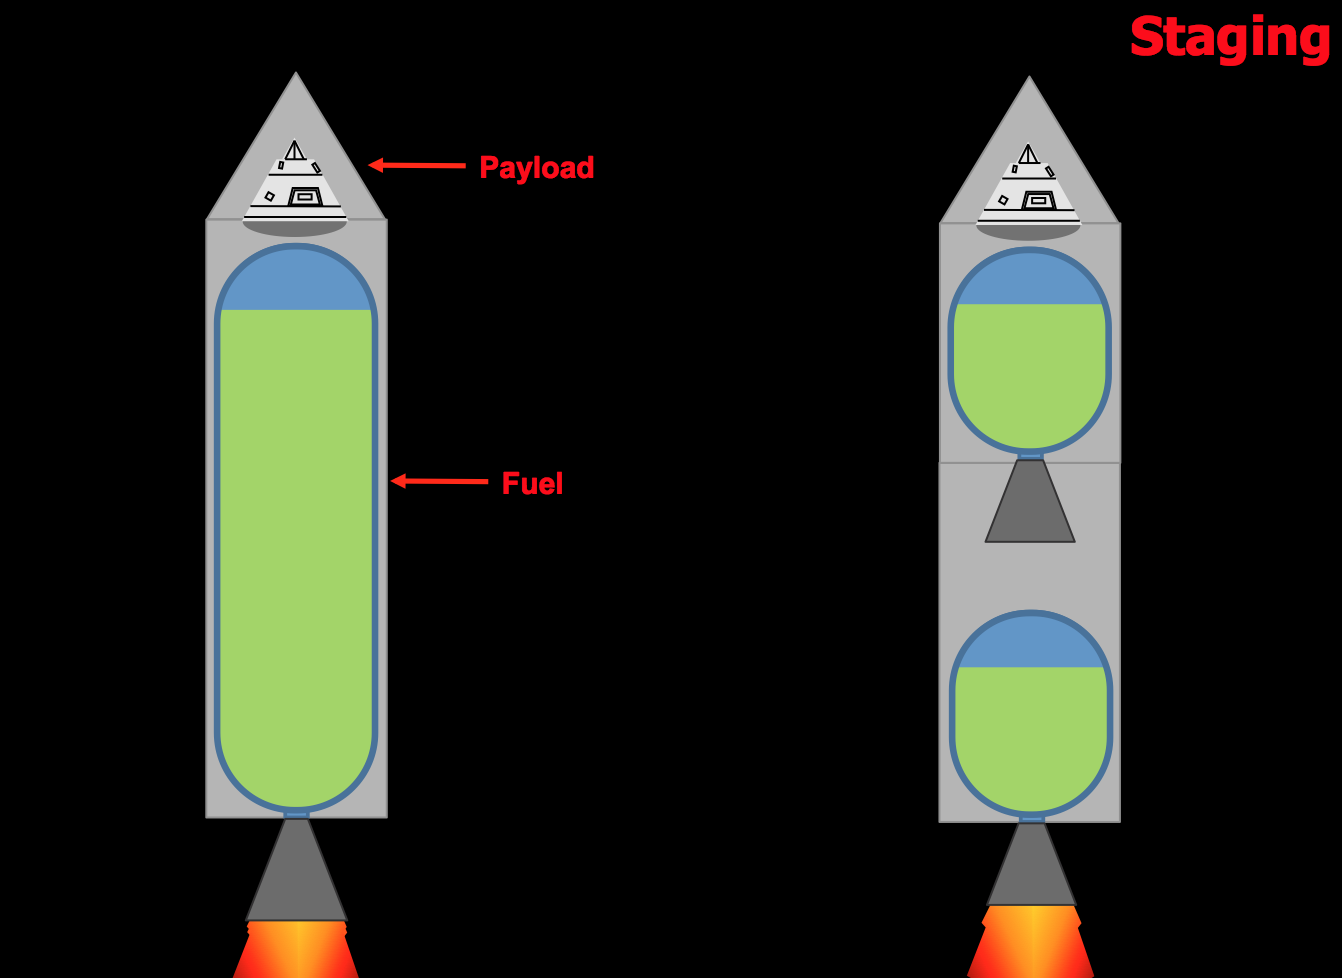
\includegraphics[width=0.5\textwidth]{images/staging1}
        \end{center}
    \end{block}
\end{frame}
\begin{frame}
    \frametitle{Staging}
    \begin{block}{}
        \begin{center}
            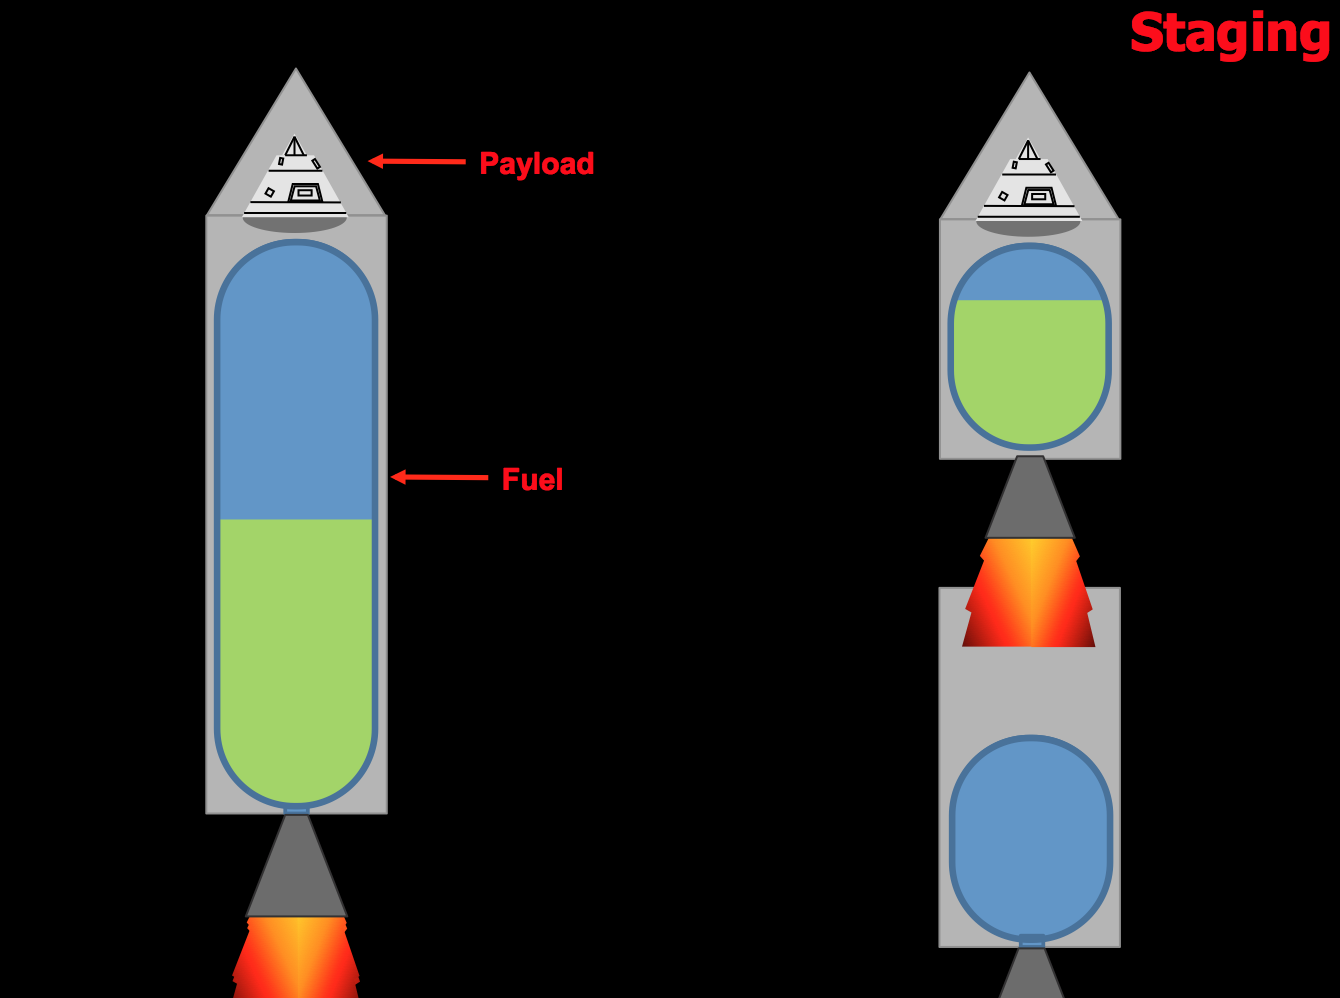
\includegraphics[width=0.5\textwidth]{images/staging2}
        \end{center}
    \end{block}
\end{frame}

{
\usebackgroundtemplate{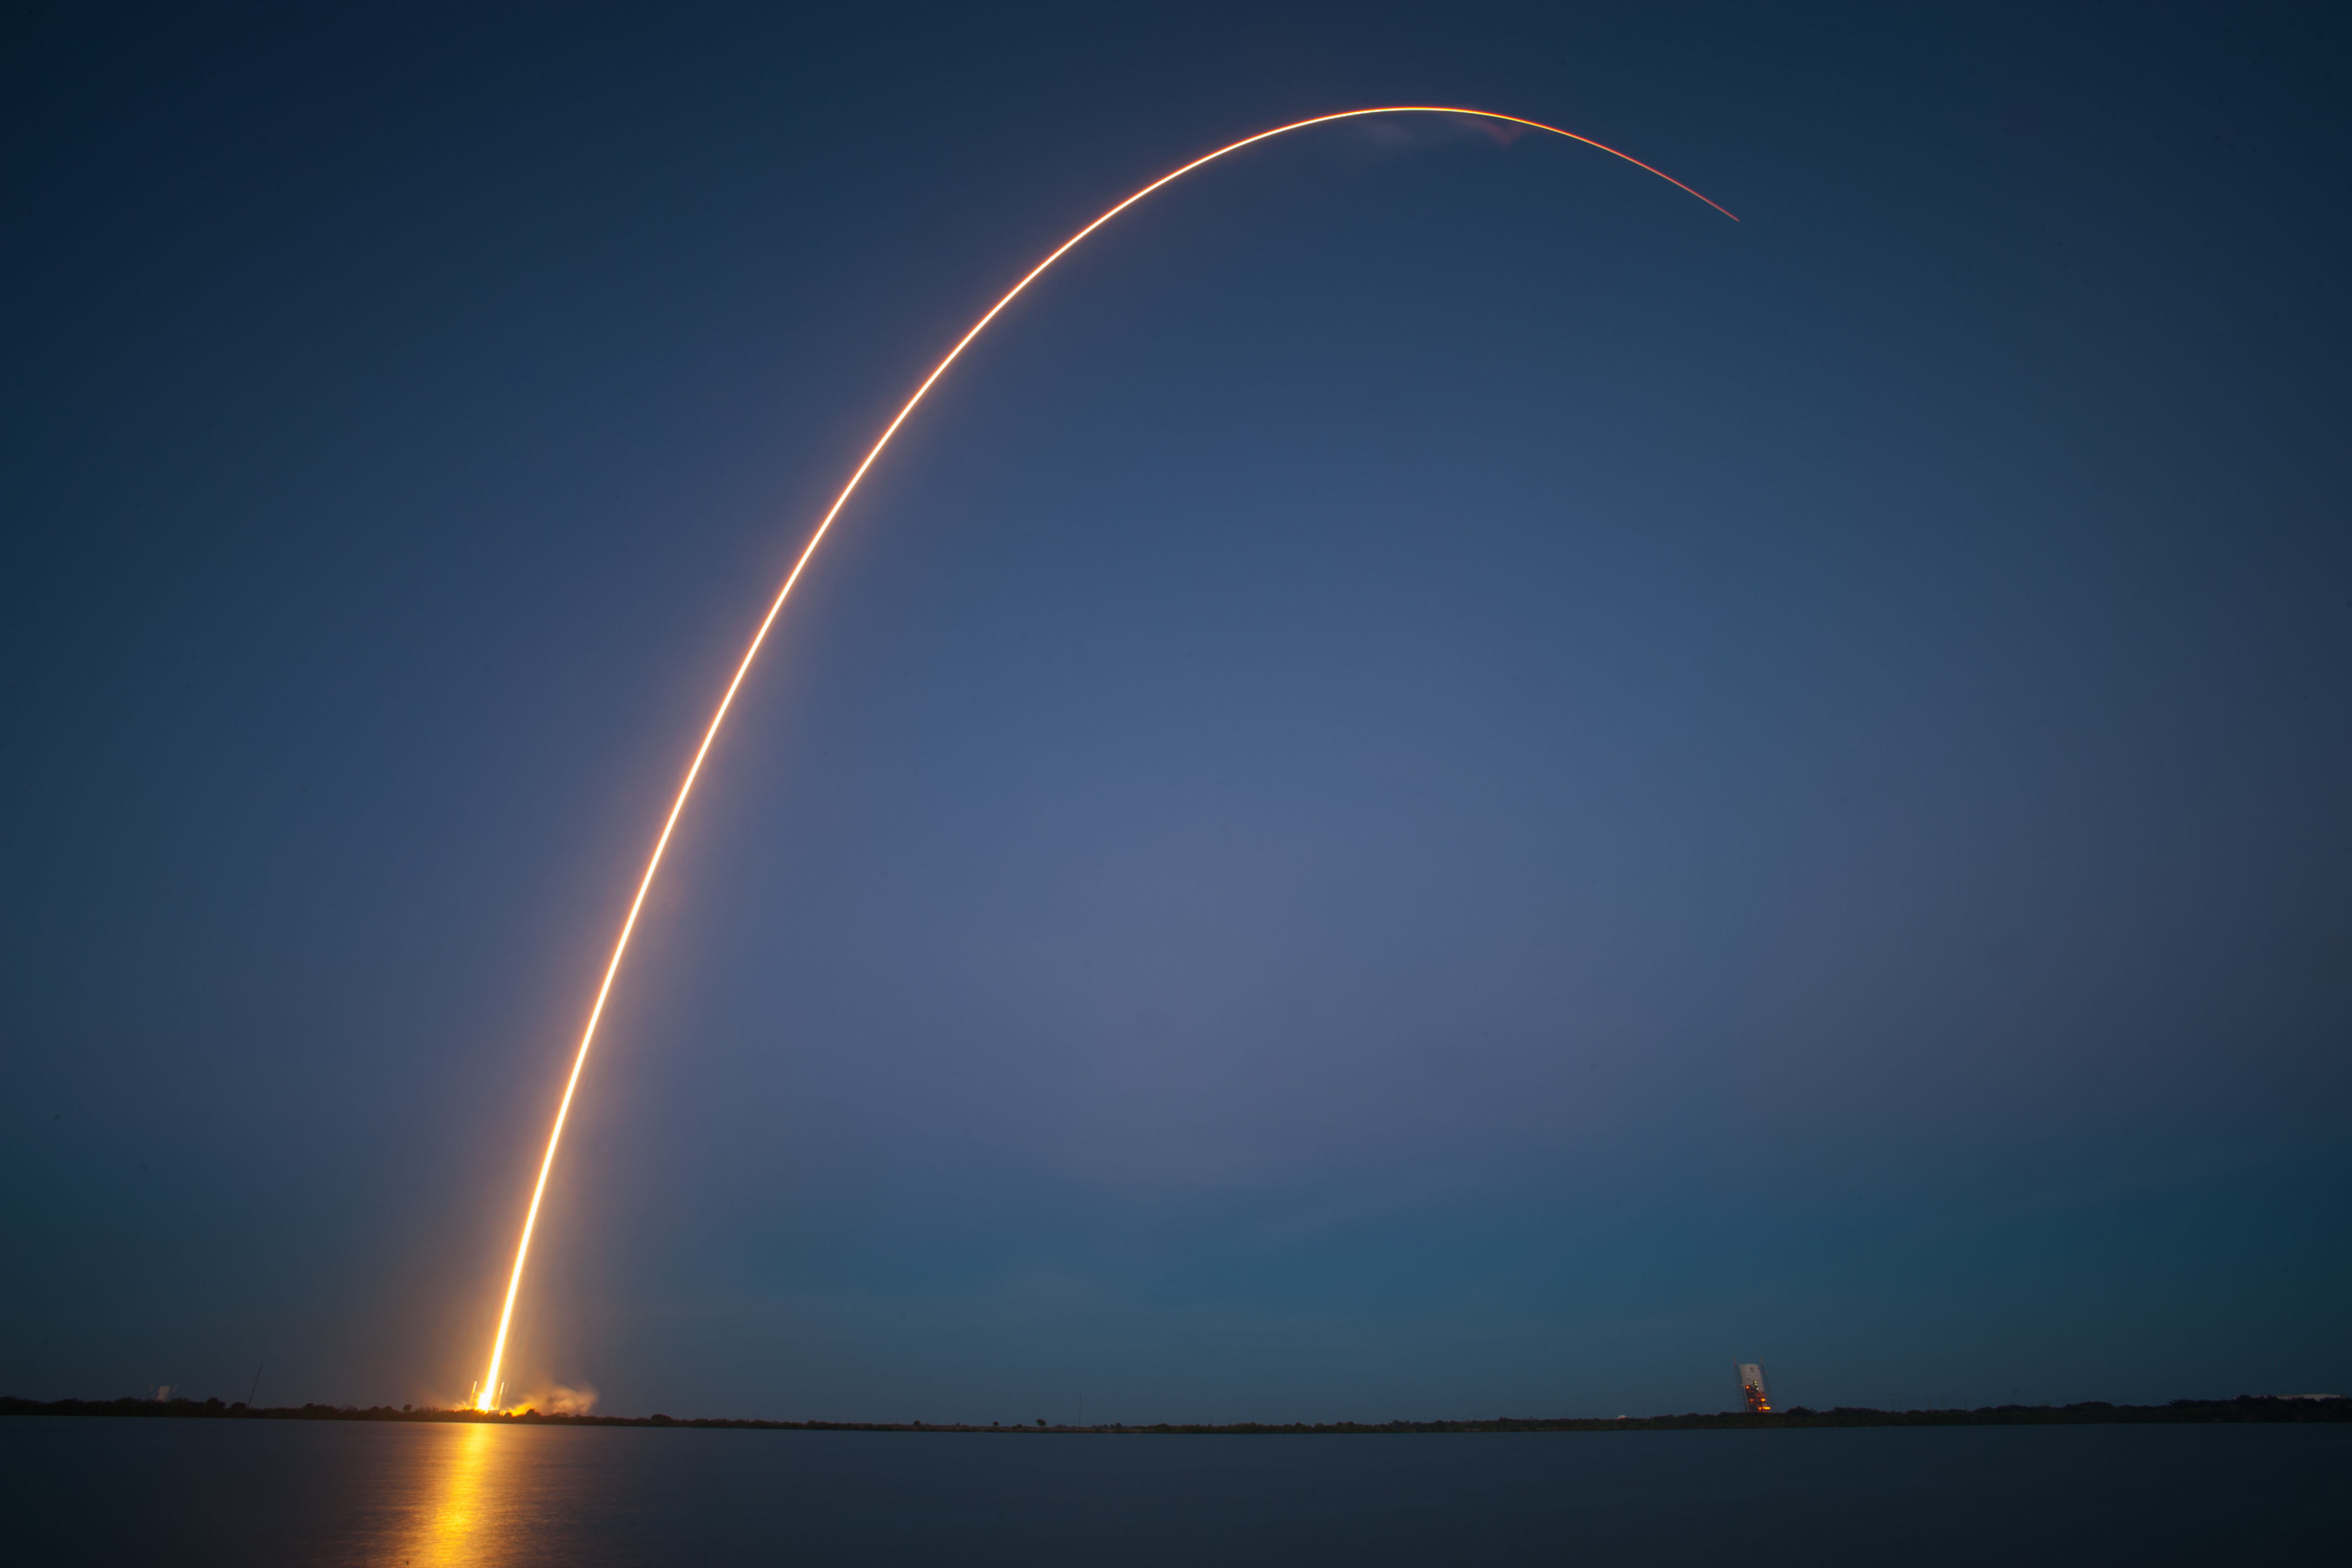
\includegraphics[height=\paperheight, keepaspectratio]{images/gravity_turn}}%
\begin{frame}
\end{frame}
\begin{frame}
    \frametitle{Getting into orbit}
    \begin{block}{Why do we turn?}
        \begin{itemize}
            \item Going straight up gains altitude quickly
            \item But we would just fall down again
            \item To get into orbit we need to move lateral as well
        \end{itemize}
    \end{block}
\end{frame}
\begin{frame}
    \frametitle{}
    \begin{block}{Gravity turn}
        \begin{itemize}
            \item Rotation of earth is already moving us towards the east at 1.5km/h. Turning east saves precious delta-v
            \item Rotational velocity is higher around the equator, so launch close to it (Cape Canaveral)
        \end{itemize}
    \end{block}
\end{frame}
\begin{frame}
    \frametitle{Let's launch!}
    \begin{block}{How do we do it?}
        \begin{itemize}
            \item Point eastward (about 5 degrees)
            \item Fire rocket
            \item Don't. Touch. Anything. Let gravity do the work
            \item Activate staging at the appropriate times
            \item Circularize orbit
            \item It's not rocket science
        \end{itemize}
    \end{block}
\end{frame}
}
